\documentclass[12pt]{report}
\usepackage{graphicx}
\usepackage[utf8]{inputenc}
\usepackage[spanish]{babel}
\usepackage{setspace}
\usepackage{geometry}
\usepackage{titlesec}
\usepackage{times}
\usepackage{mathptmx} % Use mathptmx instead of times
\usepackage{fancyhdr}
\usepackage{float}
\usepackage{pdfpages}



% Configuración de márgenes
\geometry{
    top=2.5cm,
    left=3cm,
    right=3cm,
    bottom=2.5cm
}

% Configuración de interlineado
\onehalfspacing

% Configuración de títulos y subtítulos
\titleformat{\chapter}[display]
  {\normalfont\bfseries\centering}{}{0pt}{\fontsize{14}{16}\selectfont}
\titleformat{\section}
  {\normalfont\bfseries}{\thesection}{1em}{\fontsize{12}{14}\selectfont}
\titleformat{\subsection}
  {\normalfont\bfseries}{\thesubsection}{1em}{\fontsize{12}{14}\selectfont}


% Configuración de pie de página
  \fancyhf{}
\fancyfoot[R]{\thepage}
\pagestyle{fancy}
\fancypagestyle{plain}{
  \fancyhf{}
  \fancyfoot[R]{\thepage}
}

  \begin{document}
  \pagenumbering{roman}
%----- PORTADA ----
\setlength{\hoffset}{27 pt} % 1 (Para centrar más la portada)
\begin{titlepage}
{\centering
{\fontfamily{ptm}\scshape\bfseries\fontsize{29.16}{34.992}\selectfont Universidad de Guadalajara \par}
\vspace{0.5cm}
{\scshape\Large Centro Universitario de los Lagos \par}
\vspace{1cm}
{\scshape\Large División de Estudios de la Biodiversidad e innovación Tecnológica \par}
\vspace{1cm}
{\graphicspath{{imagenes/Portada}} %ruta de las imagenes

\includegraphics[width=0.3\textwidth]{image.png}\par}
\vspace{1cm}
% Título
{\scshape\large\bfseries Practica 8: Empacado de Manzanas\par}
\vspace{0.5cm}
% Materia
{\large \textbf{Materia:} \\Controladores Lógicos Programables\par}
\vfill
% Estudiante
{\large \textbf{Presenta:} \\Oscar Iván Moreno Gutiérrez \#220942754
\\Maximiliano Frias Campos \#217488066
\par}
\vfill
% Profesor
{\large \textbf{Profesor:} \\Dr. Afanador Delgado Samuel Mardoqueo \par}
\vfill
\vfill
% Fecha
\begin{flushright}
  {\normalsize \textbf {Fecha:} \\ \today}
\end{flushright}
\vfill}
{\large  \par}
\end{titlepage}
%----- FIN DE PORTADA ----

%----- ÍNDICE GENERAL ----
\tableofcontents
\newpage

%----- PALABRAS CLAVE ----
\pagenumbering{arabic}
\chapter*{Palabras Clave}
\begin{itemize}
  \item \textbf{Contador:} Dispositivo que cuenta el número de eventos o elementos.
  \item \textbf{Banda transportadora:} Sistema mecánico que transporta materiales de un lugar a otro.
  \item \textbf{Sensor:} Dispositivo que detecta cambios en el entorno y envía la información a otros dispositivos.
  \item \textbf{Temporizador:} Dispositivo que mide y controla el tiempo de operación de un sistema.
  \item \textbf{Botón de arranque:} Interruptor que inicia el funcionamiento de un sistema.
  \item \textbf{Botón de paro:} Interruptor que detiene el funcionamiento de un sistema.
  \item \textbf{Paro de emergencia:} Mecanismo que detiene el sistema inmediatamente en caso de emergencia.
\end{itemize}
\addcontentsline{toc}{chapter}{Palabras Clave}


%\begin{itemize}

%\end{itemize}
\newpage

%----- OBJETIVO ----
\chapter*{Objetivo}
\addcontentsline{toc}{chapter}{Objetivo}
  Comprender y aplicar la funcion contador en un ejemplo: el empaquetado de manzanas.
\newpage

%----- CONTENIDO ----
\chapter{Contenido}
\section{Problema a resolver}
  En relacion a la imagen \ref{fig:imagenProblema} , una banda transportadora (Banda A) lleva cajas de carton vacias. Existe un punto donde otra banda transportadora (Banda B) ubicada a 90 grados de la Banda A, 
  deja caer manzanas sobre una caja vacia que ha llegado a este punto (detectada por el senseor S1).  En el momento en que arriba a este sitio una caja, la banda que las transporta se detiene transucrre 1.5 segundos y entonces la banda de las manzanas comienza a moverse, dejando caer manzanas sobre la caja vacia hasta hacer un total de 25 manzanas depositadas en la caja. Cada manzana que cae en la caja es detectada por el sensor S2.
  En ese momento, la banda que deja caer las manzanas se detiene y pasado 1.5 segundos, arranca la banda que transporta las cajas, llevandose la que se ha rellenado con manzanas y colocando una nueva caja vacia junto al sensor S1, repitiendo el proceso de llenar otra caja con 25 manzanas y asi sucesivamente.
  El sistema debe contar con un boton de arranque y uno de paro. Si ocurre un paro de emergencia la cuenta de las manzanas que ya se han colocado en la caja en turno no debe perderse y al presionar el boton de arranque debe continuar con la cuenta.
  \begin{figure}[H]
    \centering
    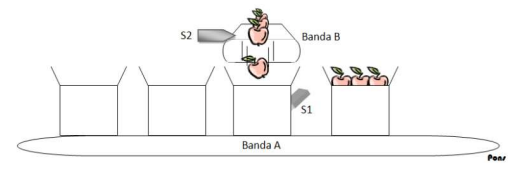
\includegraphics[width=0.5\textwidth]{screenshots/imageProblema.png}
    \caption{Imagen del problema}
    \label{fig:imagenProblema}
  \end{figure}
  \section{Diagrama de Estados}
  Se tiene el siguiente diagrama de estados:
  \begin{figure}[H]
    \centering
    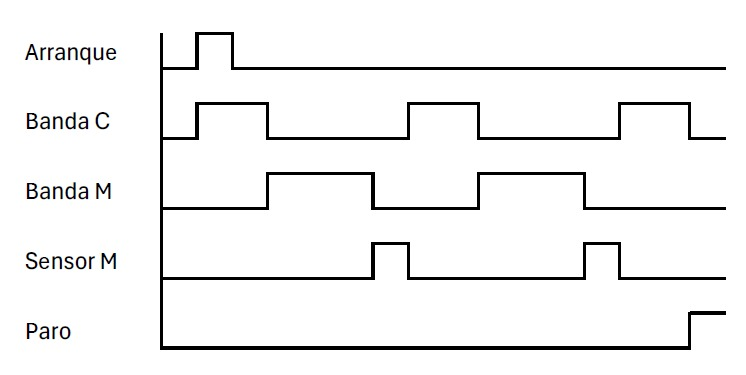
\includegraphics[width=0.5\textwidth]{screenshots/diagrama.jpg}
    \caption{Diagrama de estados}
    \label{fig:estados}
  \end{figure}


\section{Procedimiento}
\begin{enumerate}
  \item Declaramos las variables de nuestro circuito.
  \begin{figure}[H]
    \centering
    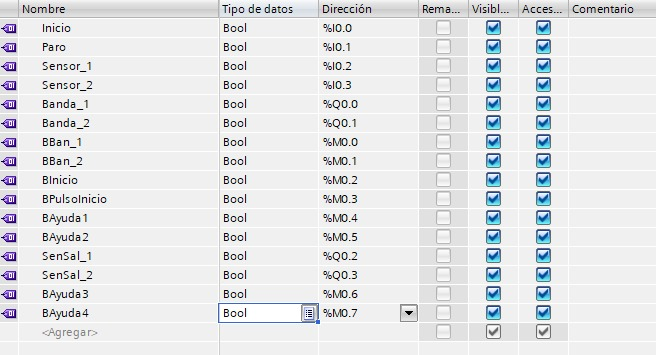
\includegraphics[width=0.5\textwidth]{screenshots/variables.jpg}
    \caption{Variables del circuito}
    \label{fig:variables}
  \end{figure}
  \item Creamos el circuito
  
\end{enumerate}

\newpage
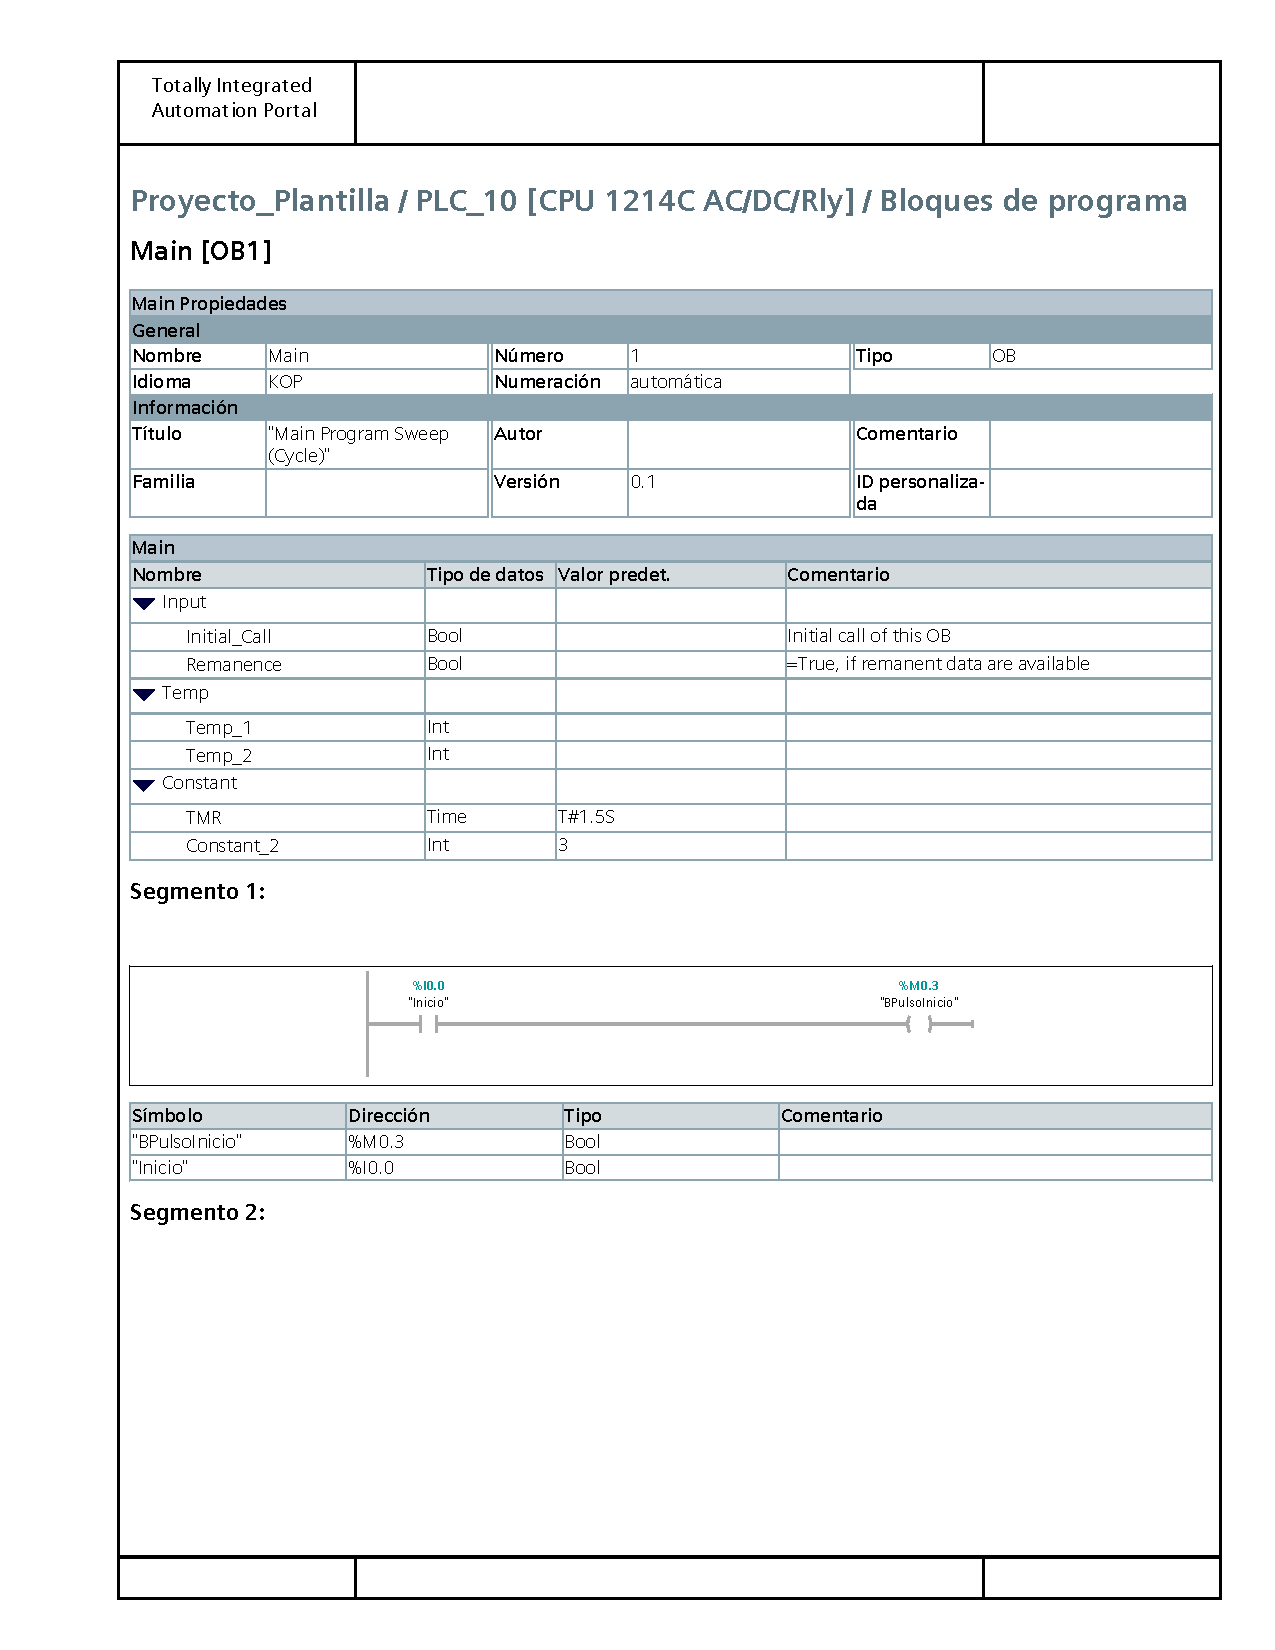
\includepdf[pages=- , offset=-40 0]{screenshots/PDF_8.pdf}
\newpage

%----- CONCLUSIONES ----
\chapter{Conclusiones}
Utilizando contadores y temporizadores TOF y TON se puede realizar un circuito que simule lo que pide el problmema anterios
\newpage


\end{document}